\documentclass[12pt,article,twosided]{memoir}
%% ::: Memoir class options for page size
%% ::: * the STOCK SIZE is LETTER
%% ::: * the TRIMMED SIZE is 6 x 9
\setlrmarginsandblock{1.25in}{*}{1}
\setulmarginsandblock{1.75in}{*}{1}
\setheadfoot{0.55in}{1in}
\checkandfixthelayout

\usepackage{polyglossia}
\setdefaultlanguage{english}
\setotherlanguage{sanskrit}
\setotherlanguage{tamil}
\setotherlanguage{telugu}
\setotherlanguage{kannada}
\setotherlanguage{malayalam}
\defaultfontfeatures{Mapping=tex-text}
\setmainfont[Numbers={Proportional},SmallCapsFont={TeX Gyre Termes},SmallCapsFeatures={Letters=SmallCaps,Numbers=Lining}]{IndUni-T}
\newfontfamily\tamilfont[Script=Tamil]{AksharUnicodeRegular}
\newfontfamily\sanskritfont[Script=Devanagari]{Jaini}
\newfontfamily\greekfont[Script=Greek]{GFS Porson}
\usepackage[shortcuts]{extdash}
\usepackage{tikz}
\usetikzlibrary{backgrounds, matrix, positioning, fadings, through}
\usepackage{pgf}
\usepackage{tipa}
\usepackage{amssymb}
\usepackage{fontawesome5}
\usepackage{totcount}
\usepackage{calc}
\usepackage{natbib}
	\bibpunct[: ]{(}{)}{; }{a}{ }{,}
\usepackage{xcolor}
\definecolor{Nesarlink}{HTML}{f6820b}
\definecolor{Nesarlinkdark}{HTML}{8a4b0b}
\definecolor{Nesarlinklight}{HTML}{fff0e0}
\usepackage{catchfile}
\usepackage{graphicx,graphbox}
\graphicspath{{images/}}
\usepackage{ragged2e}
\usepackage{tabularx}
\usepackage{changepage}
\usepackage{trimspaces}
\usepackage{framed}
\usepackage[most,breakable]{tcolorbox}
\usepackage[bottom,marginal,multiple]{footmisc}
\def\changemargin#1#2{\list{}{\rightmargin#2\leftmargin#1}\item[]}
\let\endchangemargin=\endlist 
\makeatletter
\renewcommand\@makefntext[1]{%
  \par \parindent=\z@ \noindent
  \llap{\@thefnmark.\quad}%
  {\addfontfeatures{Numbers=Lining}#1}%
}
\ExplSyntaxOn
\cs_set_nopar:Nn{\polyglossia@lang@frenchspacing:n}{\frenchspacing}
\ExplSyntaxOff
\CatchFileDef\slug{metadata/metadata-identifier.tex}{}
\CatchFileDef\doi{metadata/metadata-doi.tex}{}
\newcommand\Ndates{%
\IfFileExists{metadata/metadata-dates-submission.tex}{%
submitted \input{metadata/metadata-dates-submission.tex} {\fontspec{Noto Sans Math}⧫}}{}%
\IfFileExists{metadata/metadata-dates-acceptance.tex}{%
accepted \input{metadata/metadata-dates-acceptance.tex} {\fontspec{Noto Sans Math}⧫}}{}%
\IfFileExists{metadata/metadata-dates-publication.tex}{%
published December 8, 2024}{}
}
% TITLE COMMANDS:
% Ntitle produces Title (no subtitle)
\CatchFileDef\Ntitle{metadata/metadata-title.tex}{}
\title{\protect\trim{\Ntitle}}
% Ntitles produces Title: Subtitle
\newcommand{\Ntitles}{%
\IfFileExists{metadata/metadata-subtitle.tex}{%
{\trim{Meat Matters}}: Meat Matters}{%
Meat Matters}}
\CatchFileDef\citation{metadata/metadata-citation.tex}{}
\makeatother
\def\trim#1{\ignorespaces#1\unskip}
\newcommand{\Nyear}{\trim{2022}}
\newcommand{\Nauthor}{\trim{Jonathan Peterson}}
\author{\protect\Nauthor}
\newcommand{\article}{\trim{1}}
\newcommand{\iy}{\trim{1 (2024): 33–\total{page}.}}
\makeatother
\newcommand{\oldnums}[1]{{\fontspec[Numbers={Proportional,OldStyle}]{TeX Gyre TermesX}#1}}
\newcommand{\oldnumsbold}[1]{{\fontspec[Numbers={Proportional,OldStyle}]{TeX Gyre TermesX}\textbf{#1}}}
\setsecnumformat{\csname #1secnumformat\endcsname}
\newcommand\sectionsecnumformat{\oldnumsbold{\thesection}\quad }
\newcommand\onpage{\oldnums{\thepage}}
\newcommand{\bLozenge}{\mathbin{\blacklozenge}}

\regtotcounter{page}

% Button for CC 4.0 BY
\newcommand{\ccbylicenseButton}{%
\href{https://creativecommons.org/licenses/by/4.0/}{
\includegraphics[align=t,width=2cm]{byNesar.png}}}
% Link to journal
\newcommand{\journallink}{%
\expandafter\url\expandafter{https://nesarjournal.org/articles/\expandafter\slug}}
% Link to DOI
\newcommand{\doilink}{%
DOI: \expandafter\href\expandafter{https://doi.org/\expandafter\doi}{\doi}}
% Issue.Article (Year)
%\newcommand{\iay}{%
%\fontspec[Numbers={Proportional,OldStyle}]{TeX Gyre TermesX}issue \issue, article \article\ (\Nyear)}
% Journal logo and link
\newcommand{\brand}{%

\includegraphics[width=0.5cm,align=c]{logoNesardark.png} \hspace{0.25em} \href{https://nesarjournal.org}{\color{Nesarlinkdark}{\emph{New Explorations in South Asia Research}}}}
% Short author name (small caps, last name)
\newcommand{\shauthor}{\textsc{steinschneider}}
\newcommand\picon[1]{\raisebox{0ex}{\footnotesize{\fontspec{Printers Ornaments One}#1}}}

\makepagestyle{firstpage}
\makeevenfoot{firstpage}{\footnotesize\begin{tabular}[b]{p{5in}}%
© \theauthor\ – \emph{New Explorations in South Asia Research} \iy \\ %{\tiny\fontspec{Noto Sans Math}⧫}
\Ndates\\
\journallink\\
\doilink\end{tabular}}{}{\ccbylicenseButton\vfill}
\makeoddfoot{firstpage}{\footnotesize\begin{tabular}[b]{p{5in}}%
© \theauthor\ – \emph{New Explorations in South Asia Research} \iy \\% {\tiny\fontspec{Noto Sans Math}⧫} 
\Ndates\\
\journallink\\
\doilink\end{tabular}}{}{\ccbylicenseButton\vfill}

\makepagestyle{finalpage}
\makeevenfoot{finalpage}{}{}{}
\makeoddfoot{finalpage}{}{}{}
\makeevenhead{finalpage}{}{}{\onpage}
\makeoddhead{finalpage}{\onpage}{}{}

\captionnamefont{\footnotesize}
\captiontitlefont{\footnotesize}

\newcommand{\footer}{%
\begingroup\vfill\vspace{4ex}\noindent\begin{minipage}[t]{0.3\textwidth}
\noindent
\includegraphics[align=t,width=0.975\textwidth]{logo-wordmark.png}\\[1ex]
\resizebox{0.975\textwidth}{!}{\href{https://nesarjournal.org}{\color{Nesarlinkdark}{\texttt{https://nesarjournal.org}}}}
\end{minipage}\hfill
\begin{minipage}[t]{0.6\textwidth}
\footnotesize\raggedright\noindent{}\citation
\end{minipage}\endgroup}

\createmark{section}{both}{nonumber}{}{}
\nouppercaseheads
\makepagestyle{nesar}
\makeevenhead{nesar}{}{}{\color{Nesarlinkdark}{\thetitle \hspace{0.25em} \picon{e} \hspace{0.25em} \onpage}}
\makeoddfoot{nesar}{\brand\ \iy }{}{}
\makeevenfoot{nesar}{}{}{}
\makeoddhead{nesar}{\color{Nesarlinkdark}{\onpage \hspace{0.35em} \reflectbox{\picon{e}} \hspace{0.25em} \shauthor}}{}{}
\newtcolorbox{titlebox}[1][]{
    enhanced,
    boxrule=2pt,
    colframe=Nesarlinkdark!50!black,
    rounded corners,
    fontupper=\rmfamily,
    colback=Nesarlinklight!50!white,
    #1
    }

\newlength\drop
\newcommand*\titleM
  {%
    \begingroup
    \begin{tikzpicture}[remember picture, overlay]
      \path [bottom color = Nesarlink, top color = white, ] (current page.south west) rectangle ([yshift=-5cm]current page.east);   % Adjust the position of the logo.
    \end{tikzpicture}
    \noindent \emph{An offprint from}\bigskip

    
\includegraphics[width=0.65\textwidth]{logo-wordmark.png}
%    \AddToShipoutPictureBG*
%      {%
%        \AtPageLowerLeft
%          {%
%            \includegraphics[width=\paperwidth,height=\paperheight]
%              {example-image-duck}%
%          }%
%      }%
    \setlength\drop{0.15\textheight}%
    \begin{center}%
    \vspace*{\drop}%
    \begin{tikzpicture}[remember picture, overlay]
      \node[inner sep=0pt] (backgroundimage) at ([yshift=-2cm]current page.center) {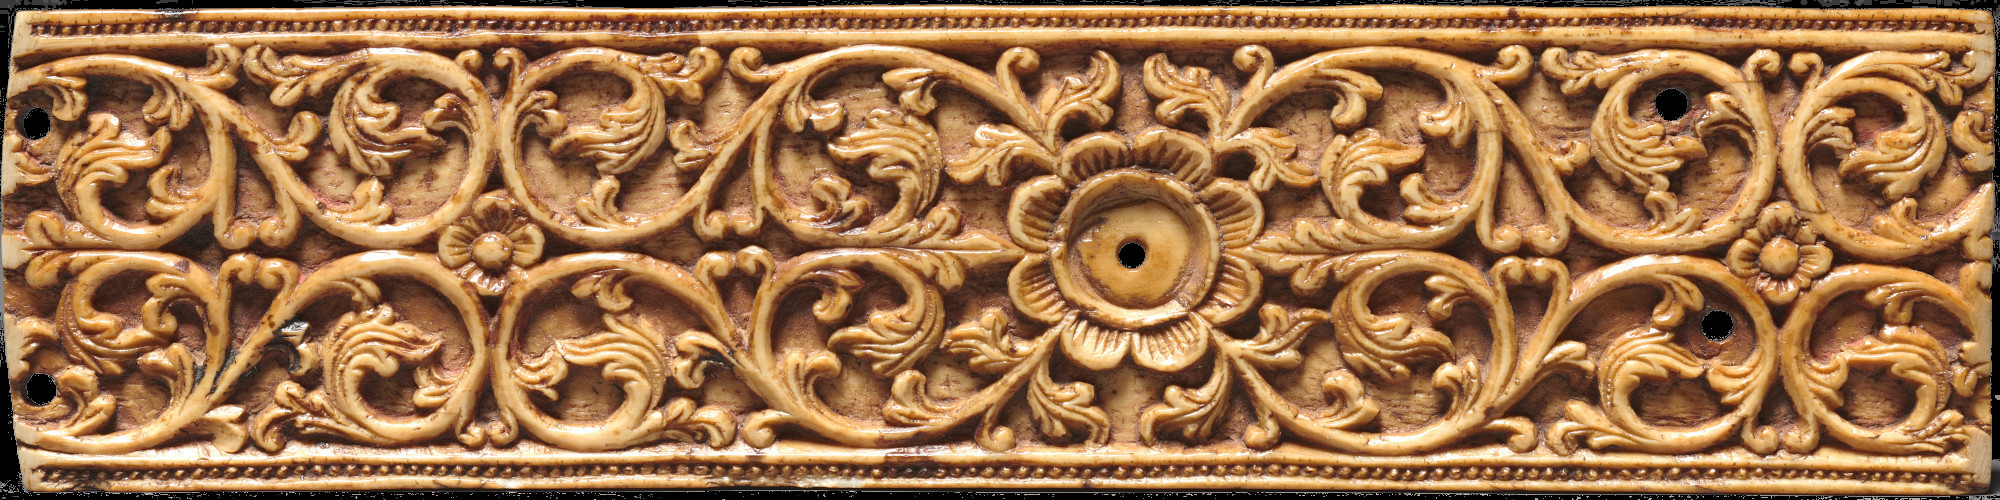
\includegraphics[width=1.2\paperwidth]{ollett-introducing-nesar.jpg}};
      \node[inner sep=0pt] (titlebox) at ([yshift=0.55cm]backgroundimage.north) {\begin{titlebox}\begin{center}\vspace{2ex}%
            \IfFileExists{metadata/metadata-subtitle.tex}{
              {\LARGE\thetitle:\par}\vspace{1ex}
              {\Large\emph{Kolaimaṟuttal} and the Genealogy of Tamil Śaiva Vegetarianism\par}\vspace{2.5ex}
            }{
              {\LARGE\thetitle\par}\vspace{2.5ex}
            }
          {\Large\textit\theauthor\par}\vspace{2ex}
          \end{center}\end{titlebox}};
      \node[inner sep=0pt] (caption) at ([yshift=1cm,xshift=-4.75cm]current page.south east) {\begin{titlebox}[add to width=-6.5cm,fontupper=\linespread{0.75}\selectfont
]%
          {\tiny\raggedright \emph{image source}: Ivory Cover of a Palm-Leaf Manuscript, Sri Lanka, 1600s, Cleveland Museum of Art (via \href{https://commons.wikimedia.org/wiki/File:Ceylon,_17th_century_-_Cover_of_a_Palm-Leaf_Manuscript_-_1992.85_-_Cleveland_Museum_of_Art.tif}{Wikimedia Commons})}%
          \end{titlebox}};

    \end{tikzpicture}
    \vfill
    %{\Large\scshape\press}%
    \end{center}%
    
    \endgroup
  }


\usepackage[linguistics]{forest}
\usepackage{pgfornament}
\usepackage{booktabs,multirow}
\usepackage{wrapfig}
\usepackage{enumitem}
\setlist[itemize]{labelindent=\parindent,itemsep=0.15em,topsep=0pt,leftmargin=\parindent}
\counterwithout{section}{chapter}
\setsecnumdepth{subsubsection}
\maxtocdepth{subsubsection}
\setlength{\cftsectionindent}{1em}
\setlength{\cftsubsectionindent}{1em}
\setlength{\cftsubsubsectionindent}{1em}
\setlength{\parindent}{2em}
\renewcommand{\cftsectionfont}{\bfseries}
\newcommand{\longmark}{{\fontspec{EB Garamond}\raisebox{0.3ex}{ː}\hspace{0.1em}}}
\newcommand{\graph}[1]{{\fontspec{Linux Libertine O}〈#1〉}}
\newcommand{\textgreek}[1]{{\fontspec{GFS Porson}#1}}
\newcommand{\phonet}[1]{{\fontspec{Linux Libertine O}\lbrack#1\rbrack}}
\newcommand{\phonem}[1]{{\fontspec{Linux Libertine O}/#1/}}
\newcommand{\mora}{{\fontspec{GFS Porson}μ}}
\newcommand{\syll}{{\fontspec{GFS Porson}σ}}
\renewcommand{\baselinestretch}{1.1}
\setlength{\RaggedRightParindent}{\parindent}
\frenchspacing
\def\nonfrenchspacing{\frenchspacing}
\AtBeginDocument{\frenchspacing}

\definecolor{formalshade}{rgb}{0.95,0.95,1}
\definecolor{darkblue}{rgb}{0.0, 0.0, 0.55}
\newtcolorbox{pullquote}{
    enhanced,
    boxrule=0pt,
    frame hidden,
    borderline west={2pt}{0pt}{Nesarlinkdark},
    colback=Nesarlinklight,
    sharp corners,
    fontupper=\rmfamily,
    left skip=24pt,
    breakable
    }
\usepackage{xurl}
\usepackage{hyperref}
\hypersetup{pdftitle=\thetitle,
        colorlinks,
        urlcolor=Nesarlink,
        linkcolor=Nesarlink,
        breaklinks=true} 
\usepackage{xurl}
\DeclareRobustCommand{\thinskip}{\hskip 0.16667em\relax}
\def\emdash{—}
\def\d@sh#1#2{\unskip#1\thinskip#2\thinskip\ignorespaces}
\def\Dash{\d@sh\nobreak\emdash}
\def\Ldash{\d@sh\empty{\hbox{\emdash}\nobreak}}
\def\Rdash{\d@sh\nobreak\emdash}

\newcounter{excounter}
\usepackage{hyphenation/nesarhyphenation}
\setcounter{excounter}{1}
\newenvironment{exe}[1]{
\begin{changemargin}{2em}{0em}\noindent\textbf{\theexcounter.\ \ #1}
\end{changemargin}
\begin{changemargin}{4em}{0em}\vspace{-1ex}\noindent\ignorespaces}%
{\end{changemargin}\addtocounter{excounter}{1}}
\widowpenalty10000
\clubpenalty10000

%\usepackage[en]{metre}
%\usepackage{gb4e}
\frenchspacing
